\documentclass{article} \usepackage{amsmath} \usepackage{amssymb} \usepackage{amsthm} \usepackage[margin=0.2in]{geometry} \usepackage{hyperref} \usepackage{physics} \usepackage{tikz} \usepackage{mathtools} \mathtoolsset{showonlyrefs} \theoremstyle{definition} \newtheorem{theorem}{Theorem}[section] \newtheorem{corollary}{Corollary}[theorem] \newtheorem{lemma}[theorem]{Lemma} \newtheorem{definition}{Definition}[section] \author{Connor Duncan} \date{\today}
\title{Physics-105-Lecture-Notes-01-31-2019}
\begin{document}
\maketitle\tableofcontents
\noindent\abstract{A single PDF with all lectures in a single document can be downloaded at \url{https://www.dropbox.com/sh/8sqzvxghvbjifco/AAC9LoSRnsRQDp7pYedgWpQMa?dl=0}. The password is 'analytic.mech.dsp'.
 This file was automatically generated using a script, so there might be some errors. If there are, you can contact me at \url{mailto:ctdunc@berkeley.edu}.}
\section{Calculus of Variations} \subsection{Euler-Lagrange Equation} \begin{equation} \dv{}{t}\dv{f}{x'}-\dv{f}{x}=0 \end{equation} describes the optimal path along some constraint, using a functional so that \begin{equation} dS=\int fdx \end{equation} Recall that if $f$ is not a function of the independent variable, ($t$ in the expression above), then you can take \begin{equation} H=y'\dv{f}{y'}-f \end{equation} and discover that \begin{equation} \dv{H}{x}=-\dv{f}{x} \end{equation} \subsubsection{Plateau's Problem, cont.} Take some soap film suspended between two hoops \begin{center} 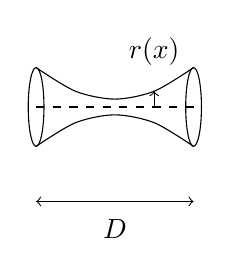
\begin{tikzpicture} \draw (-1,0) ellipse (0.1 and 0.5); \draw[dashed] (-1,0)--(1,0); \draw (1,0) ellipse (0.1 and 0.5); \draw plot [smooth] coordinates {(-1,0.5) (-.5,0.2) (0,0.1) (.5,.2) (1,0.5)}; \draw plot [smooth] coordinates {(-1,-0.5) (-.5,-0.2) (0,-0.1) (.5,-.2) (1,-0.5)}; \draw[->] (0.5,0)--(0.5,.2); \draw (0.5,1)node[anchor=north]{$r(x)$}; \draw[<->] (-1,-1.2)--(1,-1.2); \draw (0,-1.3) node[anchor=north]{$D$}; \end{tikzpicture} \end{center} surface area of a small band given by \begin{equation} dS=2\pi r(x)\sqrt{1+\left(\dv{r}{x}\right)^2}dx \end{equation} which implies that the total area is equal to \begin{equation} =2\pi\int_{-D/2}^{D/2}r(x)\sqrt{1+r'(x)^2}dx \end{equation} we can use the hamiltonian $H$ to say that \begin{equation} H=r'\dv{f}{r}-f \end{equation} with \begin{equation} \dv{f}{r'}=\frac{rr'}{\sqrt{1+r'^2}}\Rightarrow H=\frac{rr'^2}{\sqrt{1+r'^2}}-r\sqrt{1+r'^2} \end{equation} Then, take $\dv{H}{x}=-\dv{f}{x}$, so $\dv{r}{x}=\pm\sqrt{\left(\frac{r}{H}\right)^2-1}$, os we integrate \begin{equation} \int\frac{dr}{\sqrt{\left(\frac{r}{h}\right)^2-1}} \end{equation} we need to use hyperbolic cosines and sines, so we take $\frac{r}{H}=\cosh{\psi}$, which integrating gives \begin{equation} \int\frac{H\sinh\psi dr}{\sinh\psi}=H\psi \end{equation} and thus, taking $\chi=\frac{H}{D}$\footnote{don't worry, I don't totally understand how he did this integral either}. \begin{equation} r(\chi)=H\cosh\frac{\chi}{H} \end{equation} where $\chi=\frac{D}{2}, r=R$. Final result comes out to be that \begin{equation} \frac{R}{D}=\chi\cosh\left(\frac{1}{2\chi}\right) \end{equation} This is a number, which has to be equal to the geometry of the system! \subsection{Quantum $\Rightarrow$ Lagrangian Mechanics} Recall we have the transition amplitude, i.e. how probable it is to go from one state to another. \begin{equation} q_1(t_1)\rightarrow q_2(t_2) \end{equation} would be expressed as \begin{equation} \bra{q_1(t_1)}\ket{q_2(t_2)} \end{equation} which goes to \begin{align} \bra{q_2(t+\Delta t)}\ket{q_1(t)}=\bra{q_2}e^{-|\Delta H|}\ket{q_1} \end{align} we take action as \begin{equation} S(x(t))=\int_{t_1}^{t_2}dt(\frac{p^2}{2m}-V) \end{equation} then, with amplitude functional $A[x(t)]=e^{i\frac{S}{\hbar}}$, we can write an integral across every possible path, with \begin{equation} |A|^2=\int_{\text{all paths}}x(t)e^{i\frac{S(x(t))}{\hbar}}dt \end{equation} The path that wins is the one that oscillates the least, i.e. the one that has \emph{stationary phase}, since integrating an oscillator gives zero. This means we want to find a \emph{stationary} form of $S$, which is called \emph{Hamilton's Principle}, which gives that \begin{equation} \delta S(x(t))=S\int dt\left(\frac{p^2}{2m}-V\right)=9 \end{equation} \section{Lagrangian Mechanics} \subsection{Defining the Lagrangian} \begin{equation}\label{lagrangian} L=T-V \end{equation} kinetic minus potential energy. Then, the lagrangian can be put into the Euler-lagrange equation to give that \begin{equation} \dv{}{t}\dv{L}{q'}-\dv{L}{q}=0 \end{equation} which contains all of classical mechanics, since we can then write \begin{equation} S\int_{t_1}^{t_2}dtL(x,x',t) \end{equation} with mass $m$, potential $V$, we have $T=\frac{mv^2}{2}$, so the lagrangian is \begin{equation} \frac{mv^2}{2}-V(q) \end{equation} now, we write lagrange euler equation as \begin{align} \dv{L}{q'}=mq' && \dv{}{t}\dv{L}{q'}=mq'' && \dv{L}{q}=\dv{V}{q} \end{align} which gives an equation of motion \begin{equation} mq''=-\dv{V}{q}\Leftrightarrow F=ma \end{equation} \subsection{Ex: spherical pendulum} \begin{align} \vec{r}=l\cos\varphi\sin\theta\hat{x}+l\sin\varphi\sin\theta\hat{y}+l\cos\theta\hat{z}\\ \dot{\vec{r}}=(-l\dot{\varphi}\sin\varphi\sin\theta+l\cos\varphi\dot{\theta}\cos\theta)\hat{x}\\ +(l\dot{\varphi}\cos\varphi\sin\theta+l\sin\varphi\dot{\theta}\cos\theta)\hat{y}\\ -l\dot{\theta}\sin\theta\hat{z}\\ \dot{\vec{r}}\dot{\vec{r}}=l^2\dot{\varphi}^2\sin^2\theta+l^2\dot{\theta^2} \end{align} Then, we have \begin{equation} T=\frac{1}{2}m\dot\vec{r}^2=\frac{1}{2}\left(ml^2\dot\theta^2+ml^2\dot\varphi^2\sin^2\theta\right) \end{equation} Which gives a lagrangian \begin{align} L=T-V=\frac{1}{2}m\dot\vec{r}^2=\frac{1}{2}\left(ml^2\dot\theta^2+ml^2\dot\varphi^2\sin^2\theta\right)-mgl\cos\theta \end{align} Now, we want to apply the ELE, which gives two constraints \begin{align} \dv{}{t}\dv{L}{\dot\theta}-\dv{L}{\theta}=0\\ \dv{}{t}\dv{L}{\dot\varphi}-\dv{L}{\varphi}=0 \end{align} There's no $\varphi$ dependence, so \begin{equation} \dv{}{t}\left(\dv{L}{\dot\varphi}\right)=0 \end{equation} which makes it a constant of motion, so we say \begin{equation} \left(\dv{L}{\dot\varphi}\right)=p_\varphi=ml^2\dot\varphi\sin^2\theta \end{equation} We also have \begin{align} \dv{L}{\theta}=mgl\sin\theta+ml^2\dot\varphi^2\sin\theta\cos\theta\\ \dv{L}{\dot\theta}=ml^2\dot\theta\rightarrow\dv{}{t}\{dv{L}{\dot\theta}=ml^2\ddot{\theta} \end{align} Then, we can find an equaiton of motion for $\theta$, which gives \begin{equation} \ddot\theta=\frac{g}{l}\sin\theta+\varphi^2\sin\theta\cos\theta \end{equation} with another term for $\dot\varphi$, \begin{align} \dot\varphi^2=\frac{p_\varphi^2}{m^2l^2\sin^4\theta}\\ \ddot\theta=\frac{g}{l}\sin\theta+\frac{p_\varphi^2}{m^2l^2}\frac{\cos\theta}{\sin^2\theta} \end{align} Integrating this is just rude. So let's analyze some cases. \subsubsection{case $\dot\varphi=0$} implies $p_\varphi=0$, which is then \begin{equation} \ddot\theta=\frac{g}{l}\sin\theta \end{equation} which is just a regular harmonic oscillator \subsubsection{case $\dot\theta=$constant} Implies that $\ddot\theta=0$, which gives then that \begin{align} \frac{g}{l}\sin\theta+\dot\varphi^2\sin\theta_0\cos\theta_0=0\\ \left(\frac{g}{l}+\dot\varphi^2\cos\theta_0\right)\sin\theta_0=0 \end{align} if $\theta_0=0,\pi$ etc, then the pendulum is just balanced at the top, not moving. if $\cos\theta_0<0$, we have $\theta_0>\pi/2$, which gives that $\dot\varphi^2>\frac{g}{l}=\omega_0$ We could also integrate this and get complex motion, but these are the stable forms. \subsection{Driven Pendulum} \begin{center} 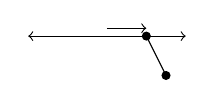
\begin{tikzpicture} \draw[<->] (-1,0)--(1,0); \draw[fill] (0.5,0) ellipse (0.05); \draw[->] (0,0.1)--(0.5,0.1); \draw[fill] (0.5,0)--(0.75,-0.5) ellipse (0.05); \end{tikzpicture} \end{center} Point on axis is being pushed, what is the motion of the point at the bottom of the pendulum? \begin{align} x=a\cos\omega t\\ r=x\hat x+l(\sin\theta\hat x-\cos\theta\hat y)\\ \dot\vec{r}=(\dot x+l\dot\theta\cos\theta)\hat x+l\dot\theta\sin\theta\hat y\\ \dot{r}^2=\dot{x}^2+l^2\dot\theta^2+2\dot x\dot\theta l\cos\theta \end{align} we set up the lagrangian \begin{align} L=T-V=\frac{1}{2}m(\dot x^2+l^2\dot\theta^2+2\dot x^2\dot\theta^2l\cos\theta)+mgl\cos\theta \end{align} and try to find simple solutions.
\end{document}
